\section{KDB arrangement and cabling}
\label{sec:DB}

In this section we describe the KDB arrangement, in-vessel cabling and external cabling. A scheme of the cabling is shown if 
figure \ref{fig:cabling:scheme}). 

\begin{figure}[ht]
    \bigskip
    \begin{center}\leavevmode
        \rotatebox{0}{
        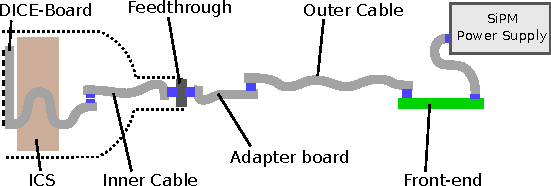
\includegraphics[width=.8\textwidth]{Simple.pdf}}
        \caption{\textit{Tracking plane cabling scheme.}}
        \label{fig:cabling:scheme}
    \end{center}
\end{figure}

\subsection*{Kapton DICE-Boards (KDBs) and in-vessel cabling}

The KDBs  where mounted on top of a thin plate of copper held by springs to the main copper plate that acts as a shielding. The reason of those springs is that they will allow for a small movement of the plate during the assembly and when closing the detector allowing for a perfect match of the tracking plane with the EL region. Fig. \ref{fig:spring_detail} shows the detail of one of those springs.

\begin{figure}[h!]
\begin{center}
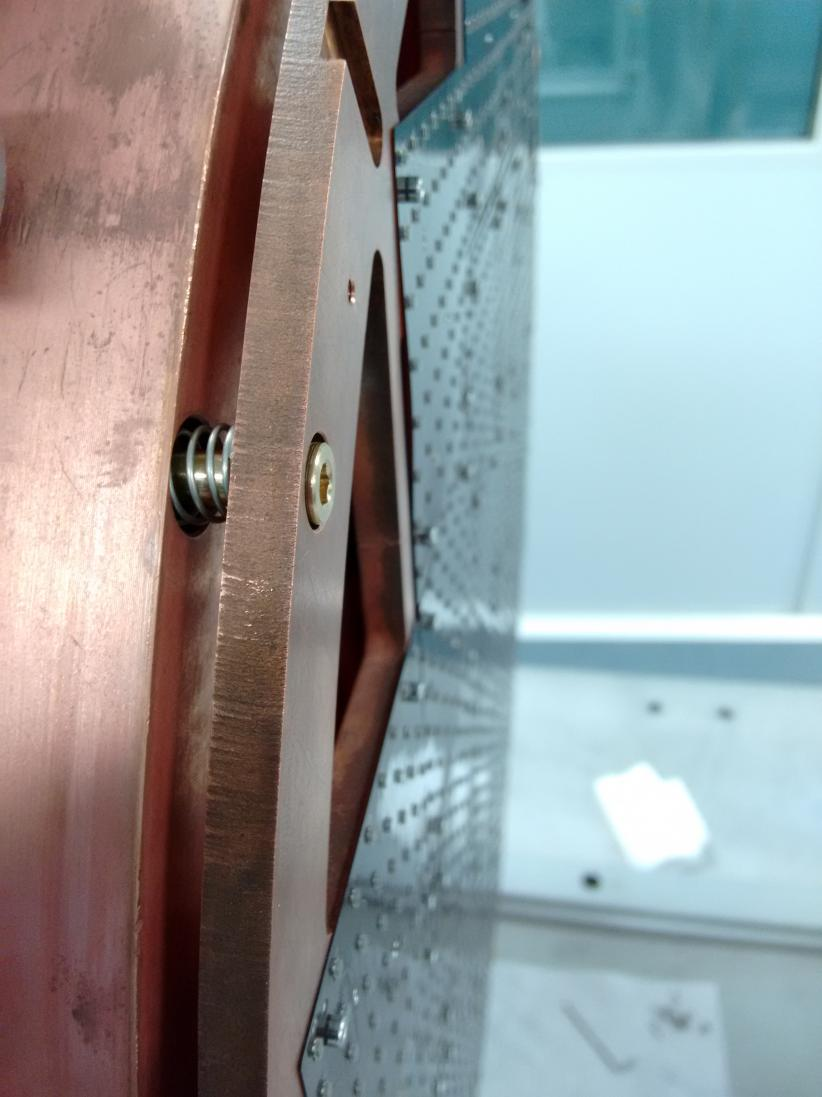
\includegraphics[width=0.45\textwidth]{IMG/spring_plate_detail}
%\hspace{15mm}
%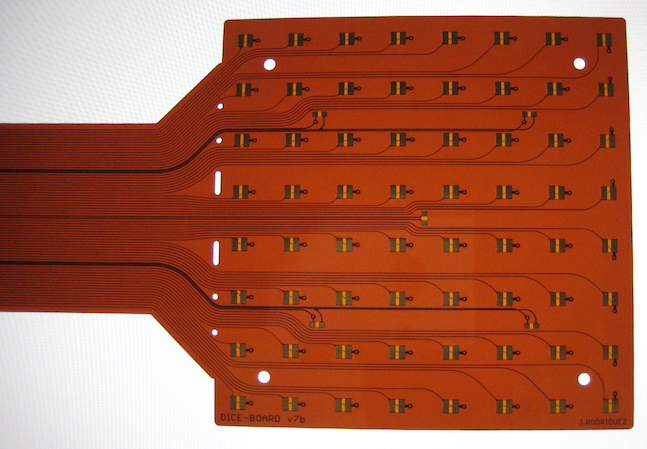
\includegraphics[width=0.39\textwidth]{IMG/DB.JPG}
\caption{Detail of one of the springs in the tracking plane thin plate that will allow to accomodate the tracking plane perfectly parallel to the electroluminescence region.}
\label{fig:spring_detail}
\end{center}
\end{figure}

Once the KDBs are mounted the tail has to be passed through the holes in the shielding plate (Fig. \ref{fig:cabling}). At the end of the tail a connector is soldered to plug a cable extension made of the same materials than the DICE-Boards. Those cables have to be organised to reach 5 different feed-throughs. The distribution of the cables is done using 3D printed structures placed inside a steel structure that will allow to extract the SiPMs cables and also is the point where the piping for vacuum and evacuation connects (Fig. \ref{fig:cabling_spaceship}).


\begin{figure}[h!]
\begin{center}
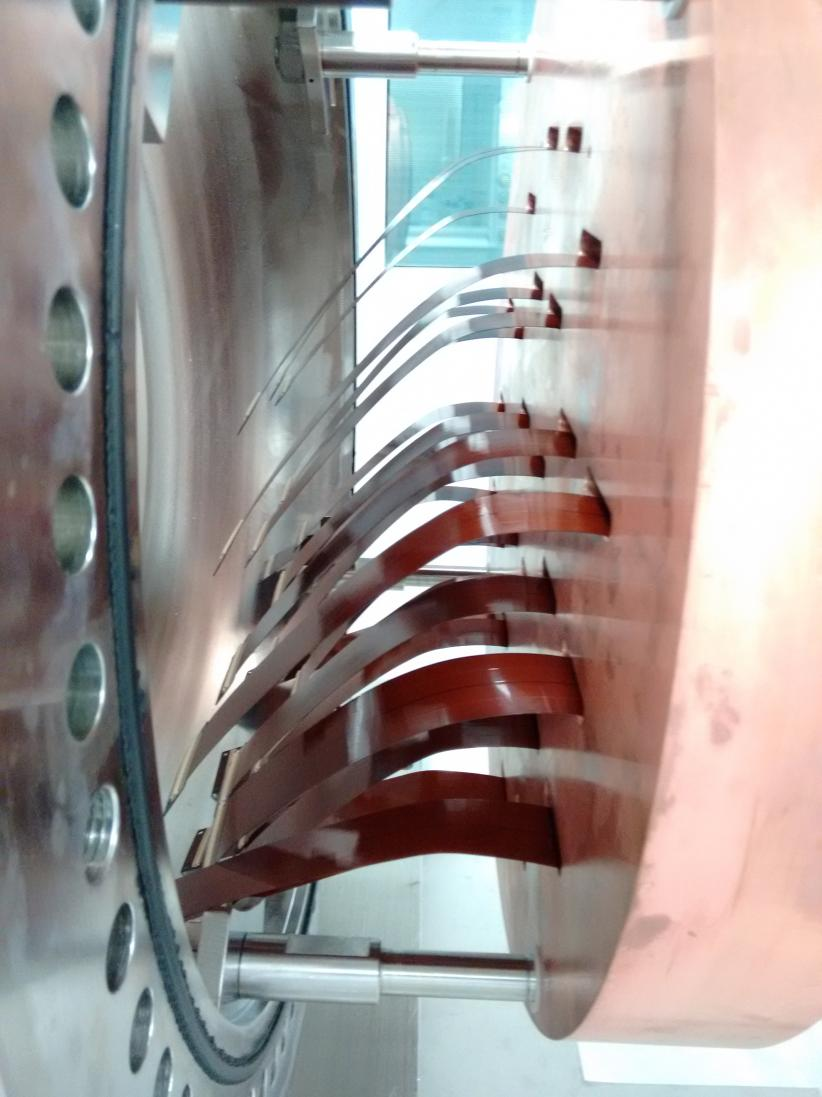
\includegraphics[width=0.45\textwidth]{IMG/cabling}
\caption{Dice-Boards cables passing through the holes in the shielding plate. At the end of the tail there is a connector that will allow for an extension of the cable to reach the feed-through.}
\label{fig:cabling}
\end{center}
\end{figure}

\begin{figure}[h!]
\begin{center}
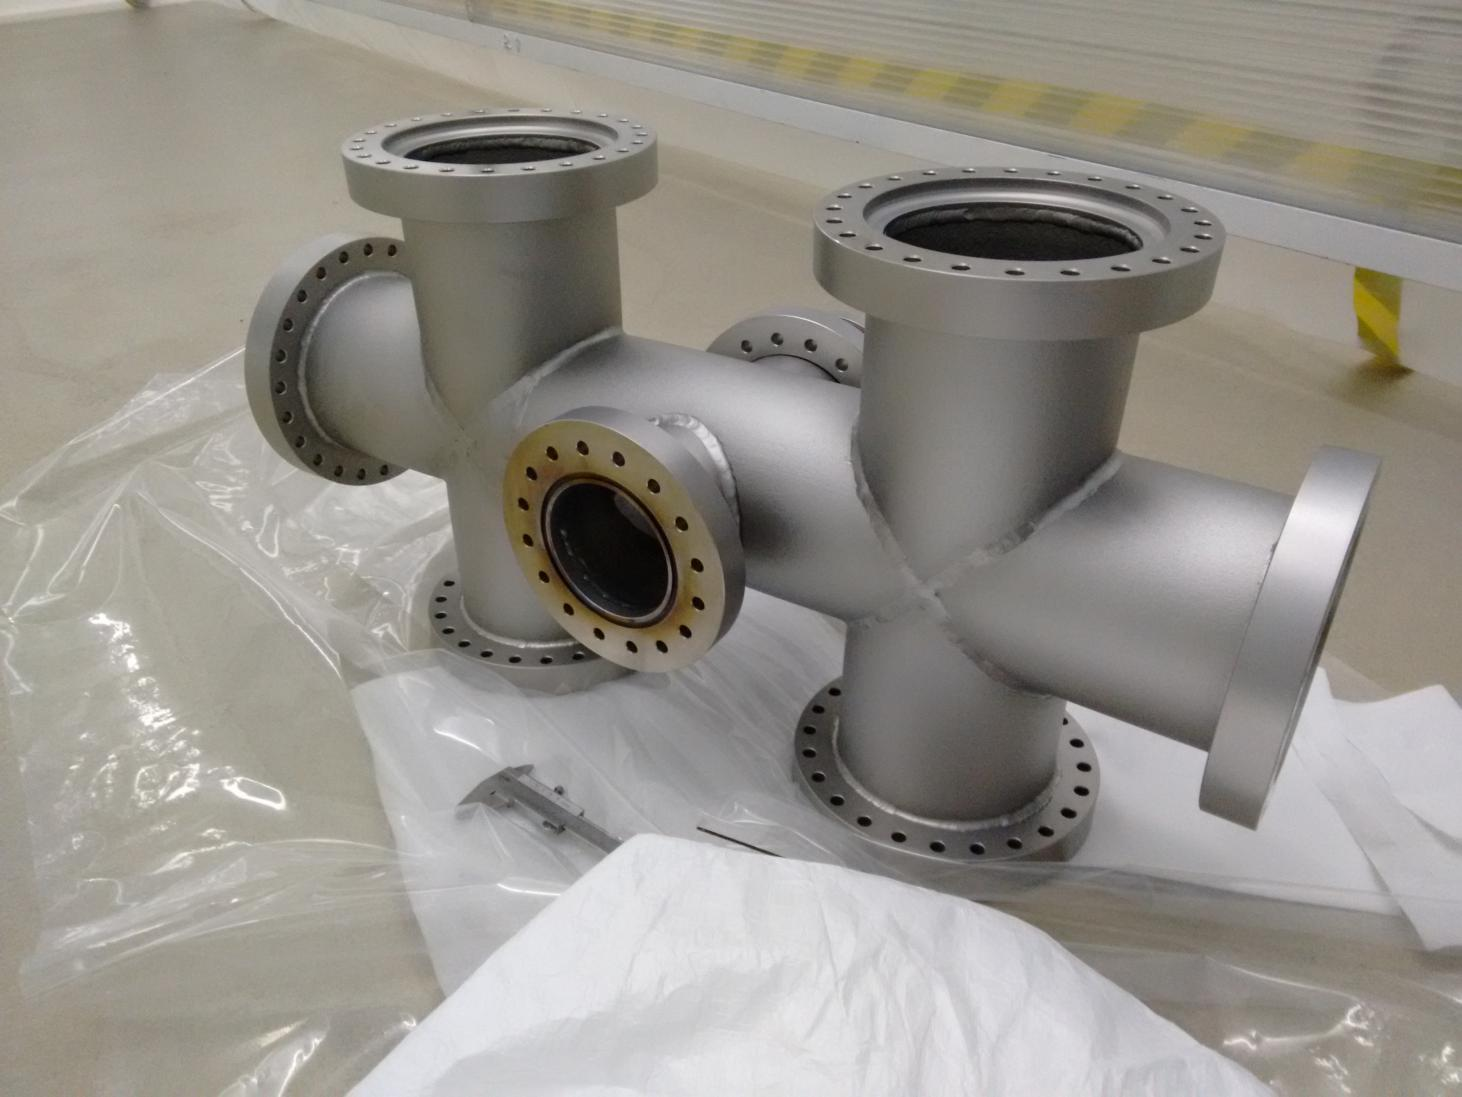
\includegraphics[width=0.45\textwidth]{IMG/spaceship_unmounted}
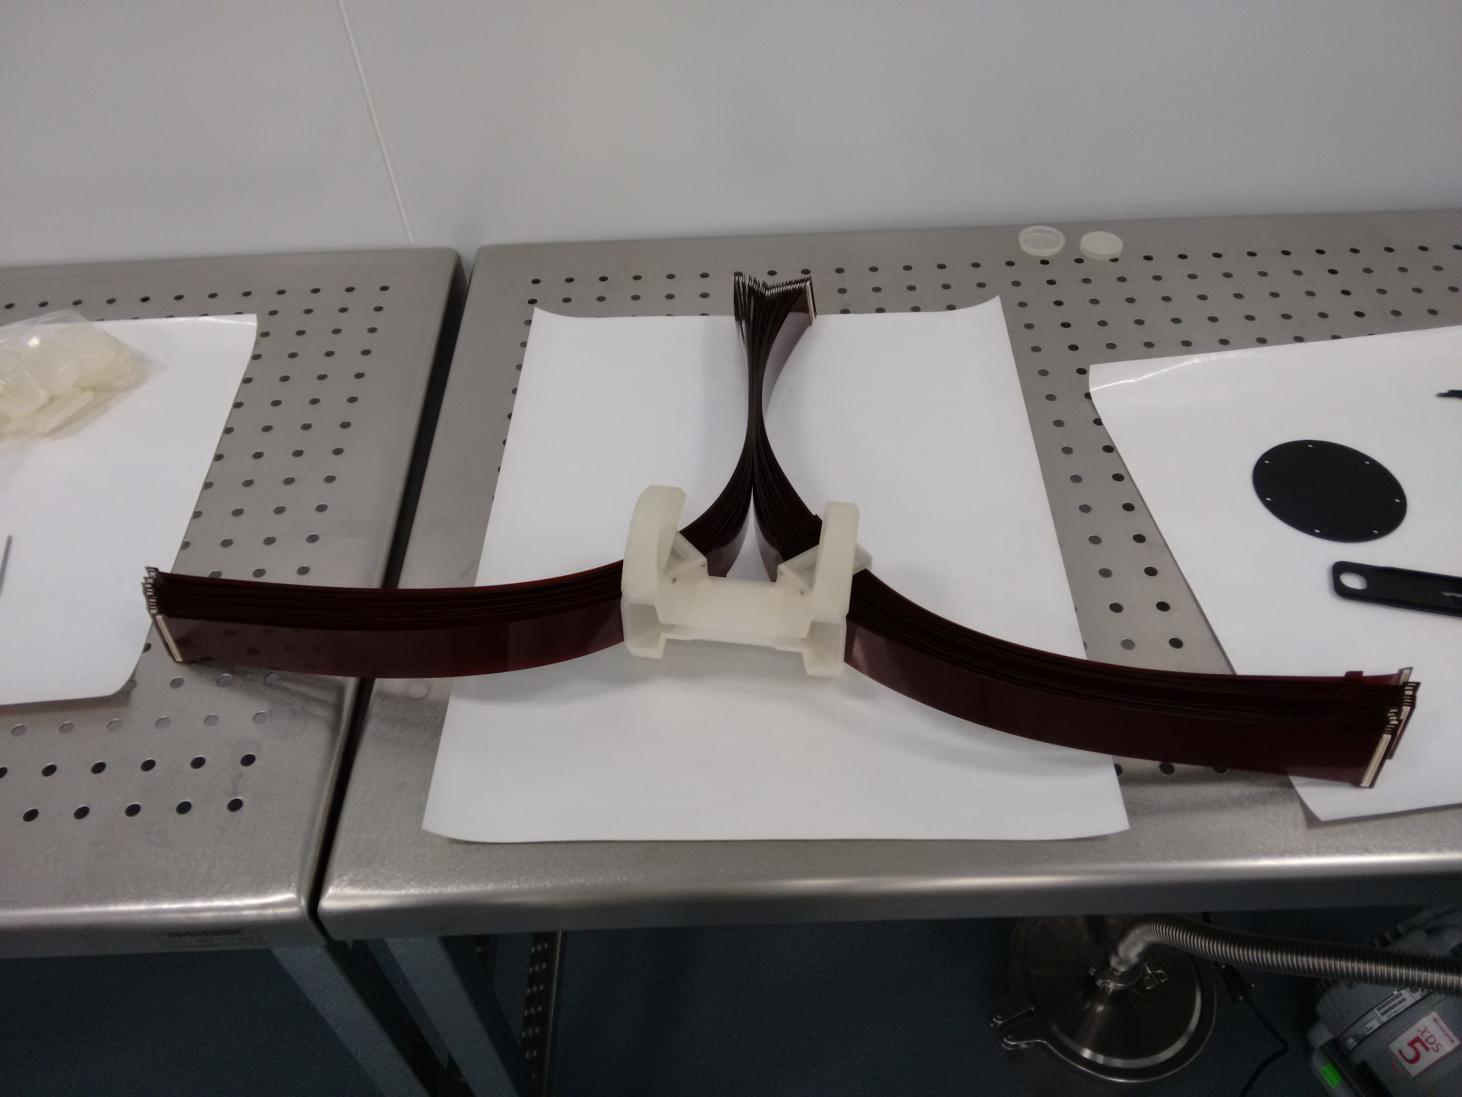
\includegraphics[width=0.45\textwidth]{IMG/spacechip_cabling}
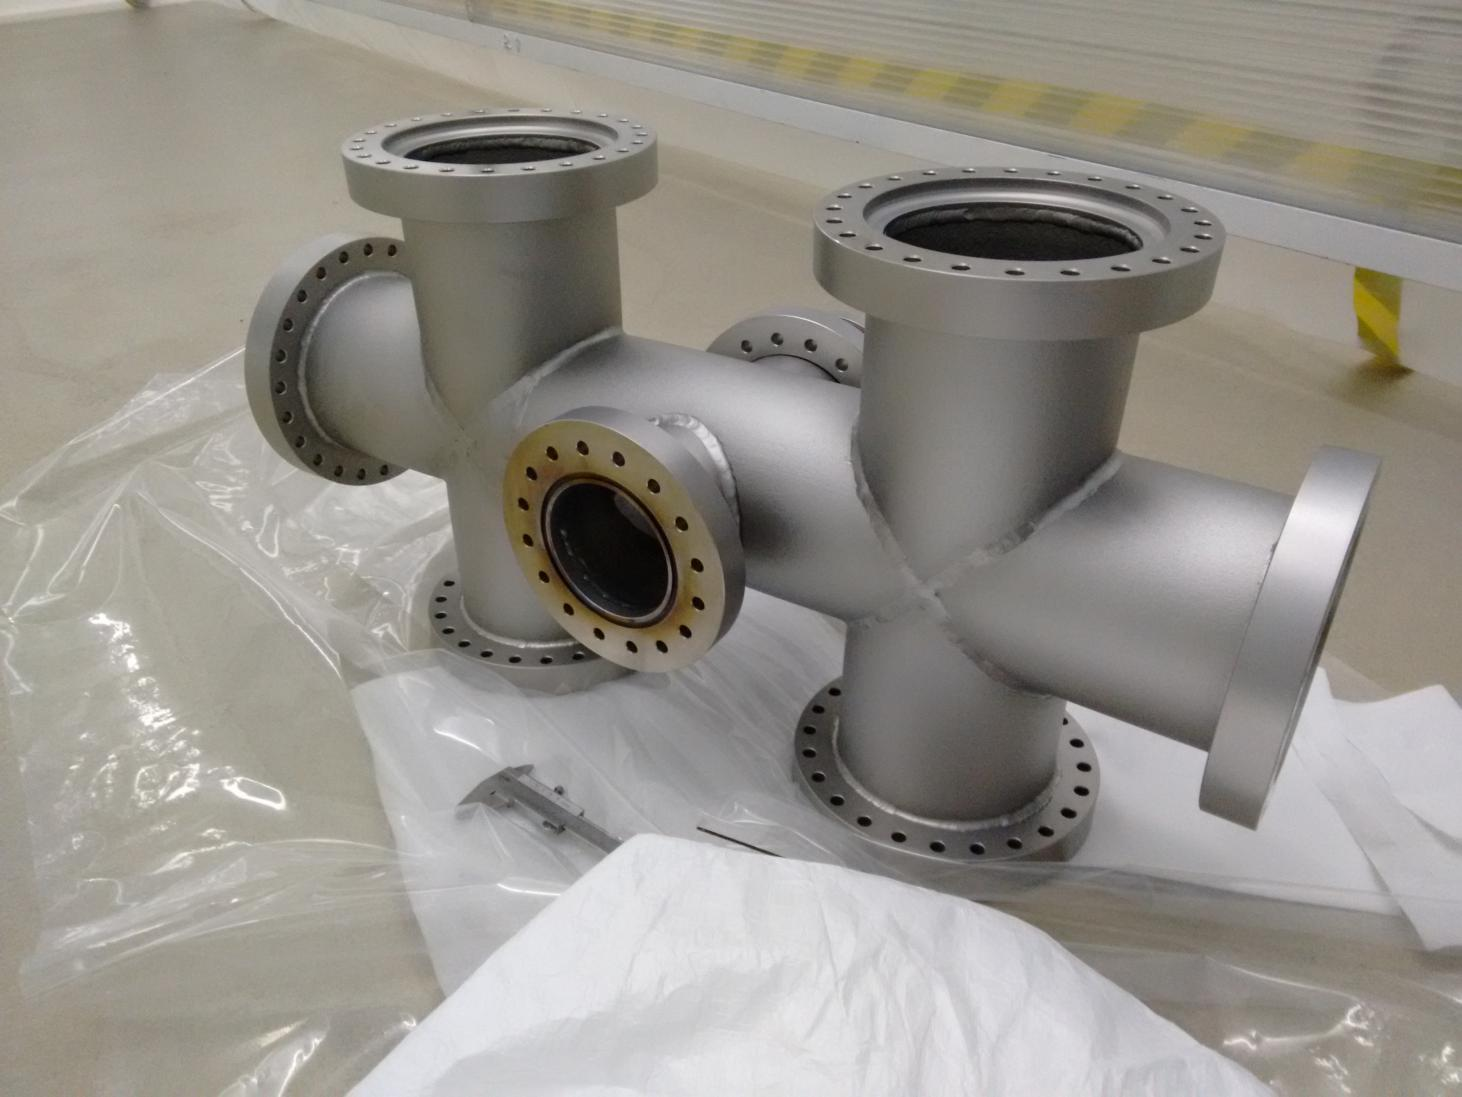
\includegraphics[width=0.45\textwidth]{IMG/spaceship_unmounted}
\caption{Up left: Steel structure to support and organize the SiPM cabling. Up right: 3D printed structure to allow a better distribution of the cables. Bottom: Assembly process of the SiPM cables.}
\label{fig:cabling_spaceship}
\end{center}
\end{figure}

The final step in the connection of inner cables of the tacking plane is the connexion to the tracking-plane feedthroughs (TPFT). Each one of these custom-made FTallows up to 6 KDB connexions. Extracting the signals of the 29 KDBs require then  5 TPFT. Figure \ref{fig:TPFT} shows the front and the back side of theTPFT as well as the cable connexion.

\begin{figure}[h!]
\centering
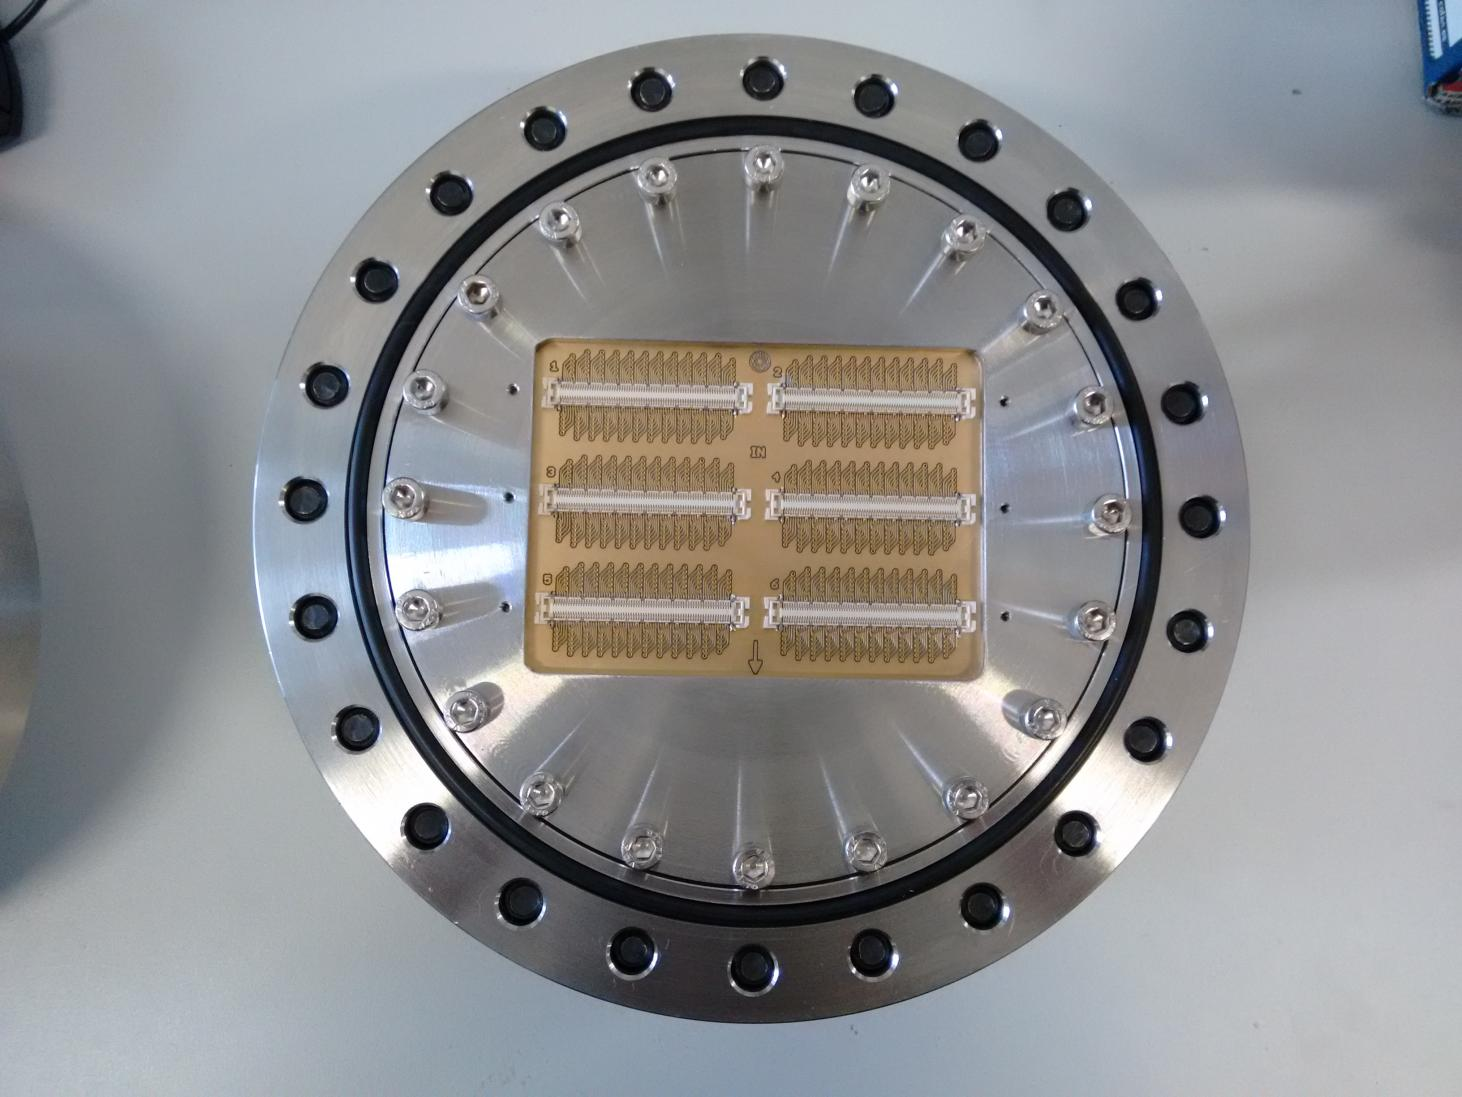
\includegraphics[width=0.45\textwidth]{IMG/TPFT1}
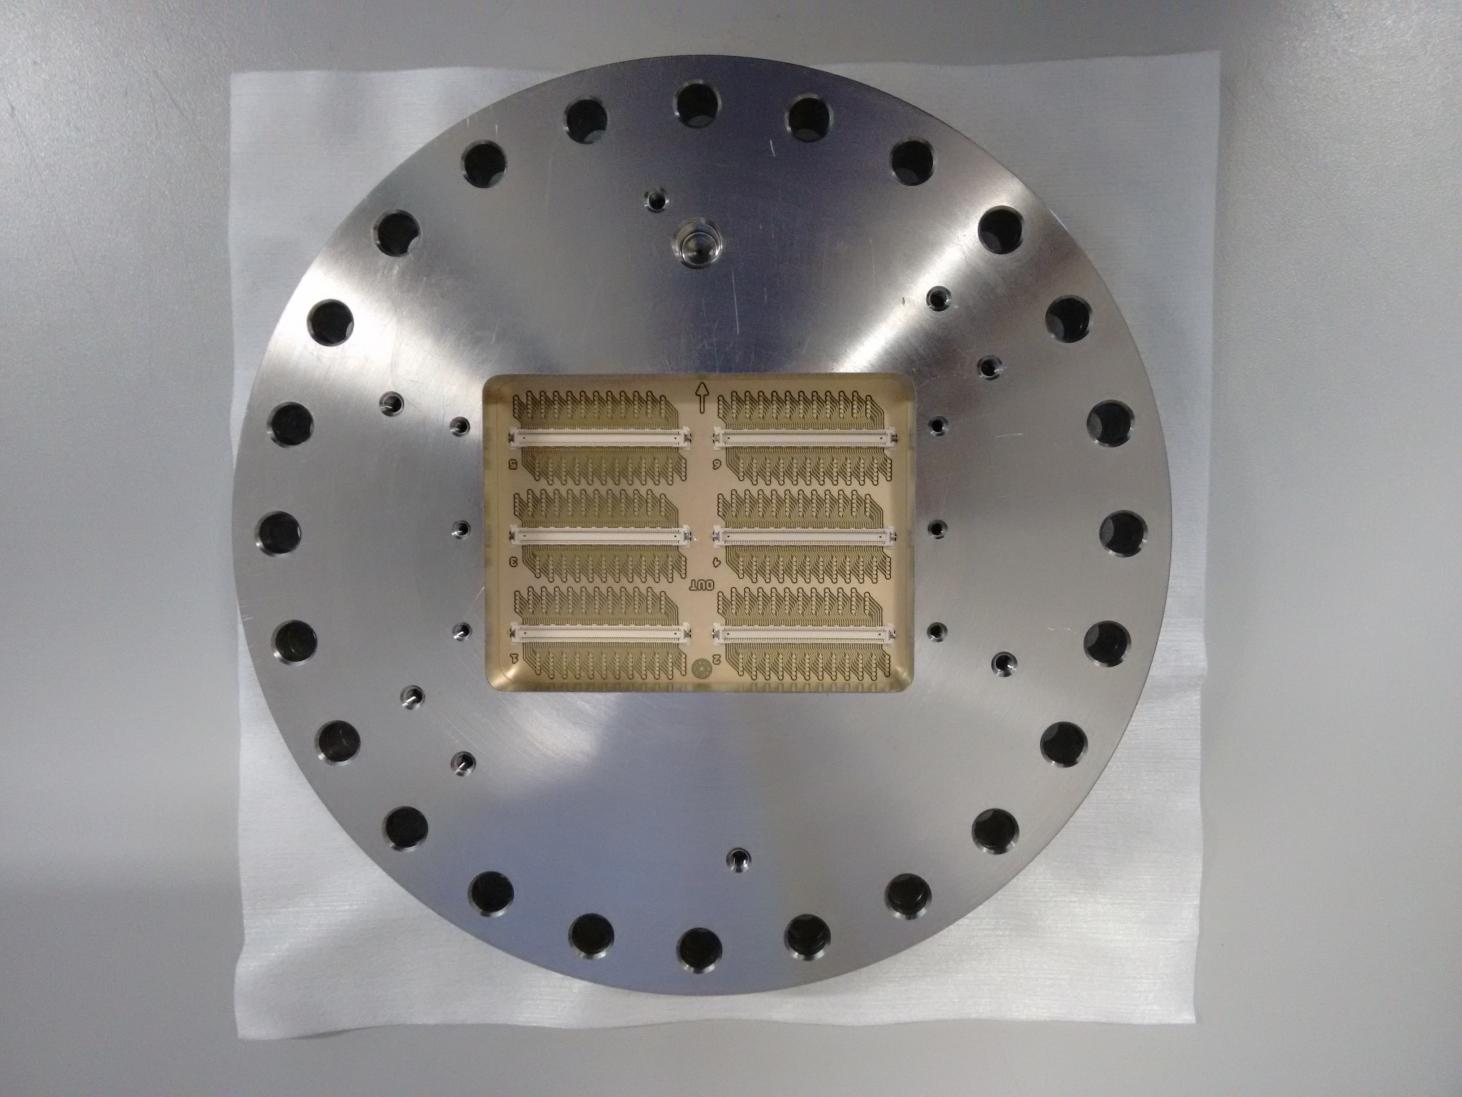
\includegraphics[width=0.45\textwidth]{IMG/TPFT2}
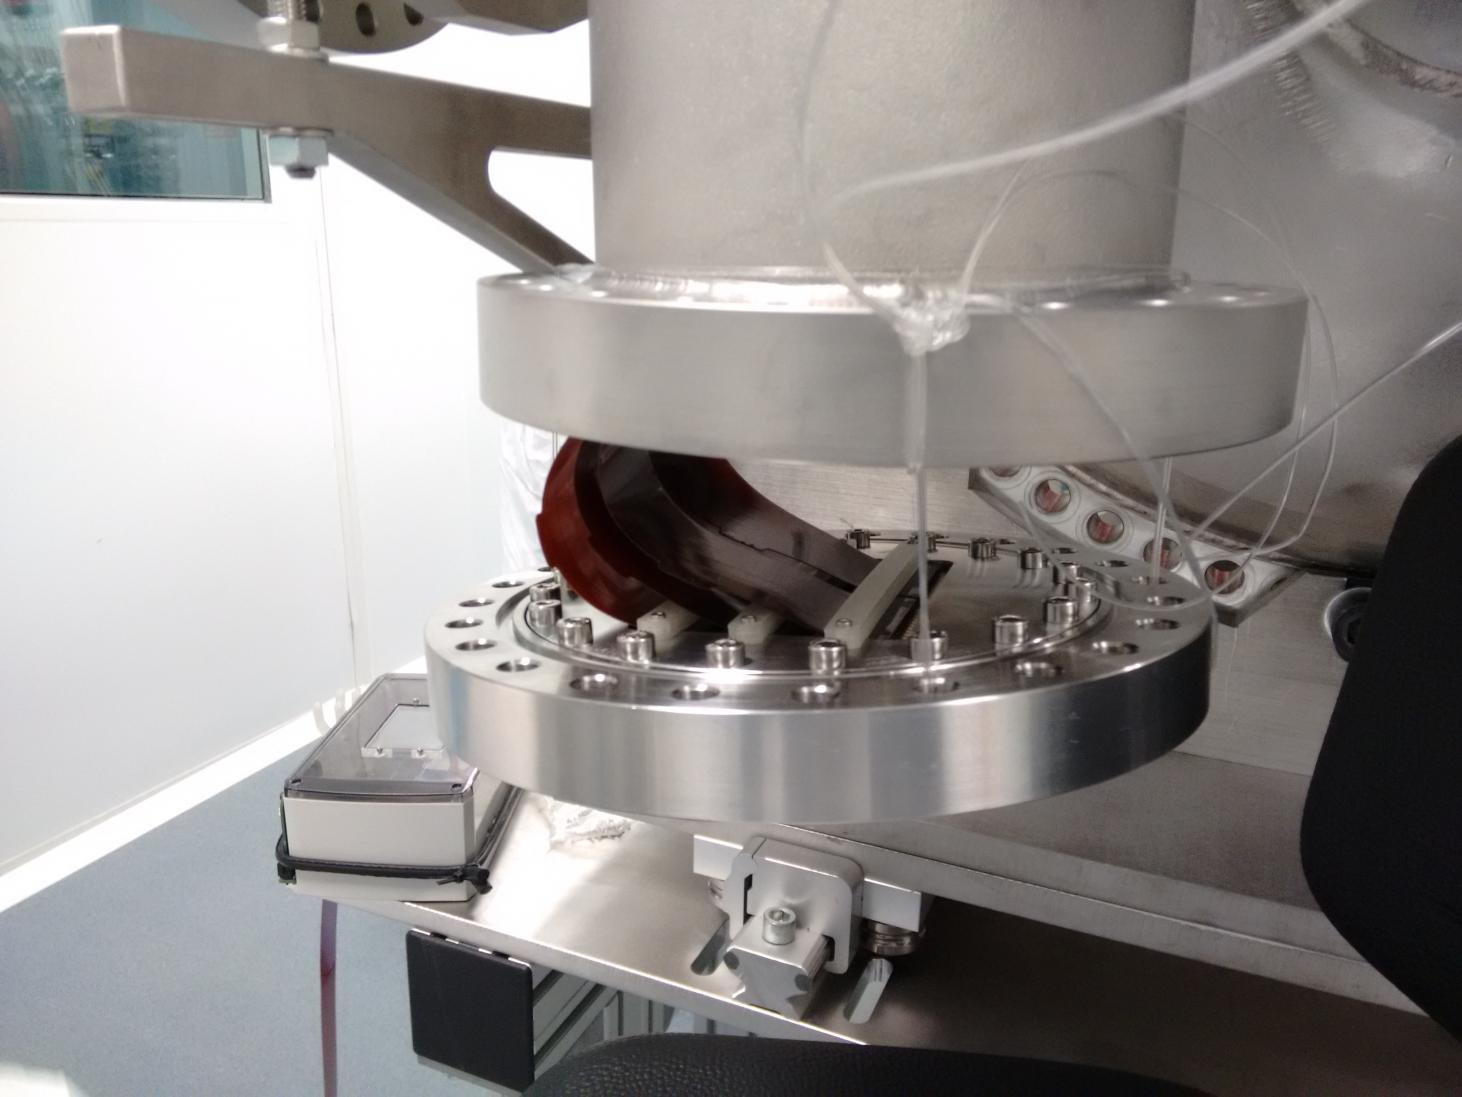
\includegraphics[width=0.45\textwidth]{IMG/TPFT_connected}
\caption{Up left: Inner side of the TPFT. Up right: external side of the TPFT. Bottom: Cable connexion.}
\label{fig:TPFT}
\end{figure}



\subsection{External cabling}\label{sec:ext}
In order to keep background events to a minimum, front-end electronics are placed nearby the detector but beyond the lead castle that surrounds the TPC, with a total cable length of $\sim$ 5 m from the sensor to the electronics. This poses a challenge in the design of a cabling solution that (1) is radio-clean enough to be inside the detector, (2) keeps enough signal-to-noise ratio in the relevant signal bandwidth for the gated integrator with a 5 m cable, (3) is cost-effective, (4) includes SiPM biasing voltage wires and (5) is also valid for the final NEXT phase (NEXT-100).

Differential transmission lines on fine-pitch FFC cables outside the detector were chosen as a good trade off between performance and cost. As shown in figure \ref{fig:external}, the cables are 0.5 mm pitch with $280 \times 76 \mu$m traces embedded in a thin polyester layer. The anode and the cathode of each SiPM are connected to the \textit{signal} and \textit{bias} lines respectively. Channels are separated by a guard trace connected to the analog ground in the front-end. Therefore three lines are needed for each SiPM channel. In addition, each KDB adds several more lines, for the  temperature sensor and  calibrating LEDs.

\begin{figure}[h!]
\centering
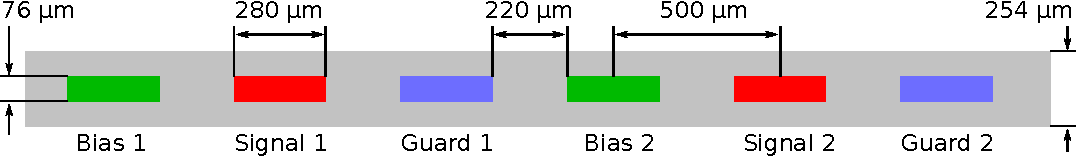
\includegraphics[width=.6\textwidth]{IMG/section.pdf}
\caption{Cross-section of the external cable (just two channels are shown).}
\label{fig:external}
\end{figure}

Since ommercial cables with the required density of traces were not available, the adopted solution was to split into four FFC cables. This way, the signals of a whole DICE-Board are distributed in four cables of 51 wires each. This distribution is done just at the output of the feedthrough, using a Kapton adapter board. This board has the same stackup as the DICE-Board or the inner cable, and splits the signals in four \textit{DF9 Hirose} connectors for the long cables.

In order to further reduce the noise coupled to the external cables, they are wrapped with a 1 mm aperture mesh, also connected to the analog ground at the front-end. This mesh is has its maximum attenuation rated at 1 MHz, which covers the range of frequencies we want to attenuate.

The external cables cables have been connected to the output of the TPFT and then they go below the platform until the position of the FEE boards where they are connected. (Fig. \ref{fig:external_installation})


\begin{figure}[h!]
\centering
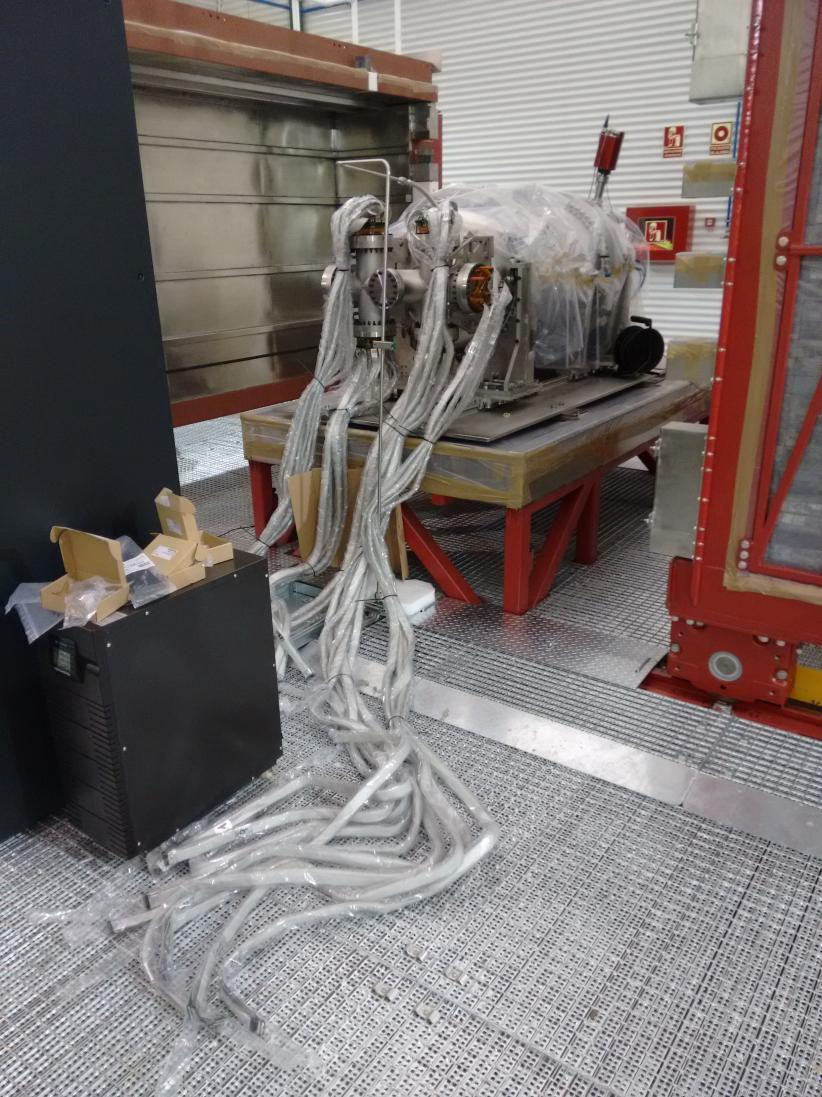
\includegraphics[width=.45\textwidth]{IMG/external_cabling2}
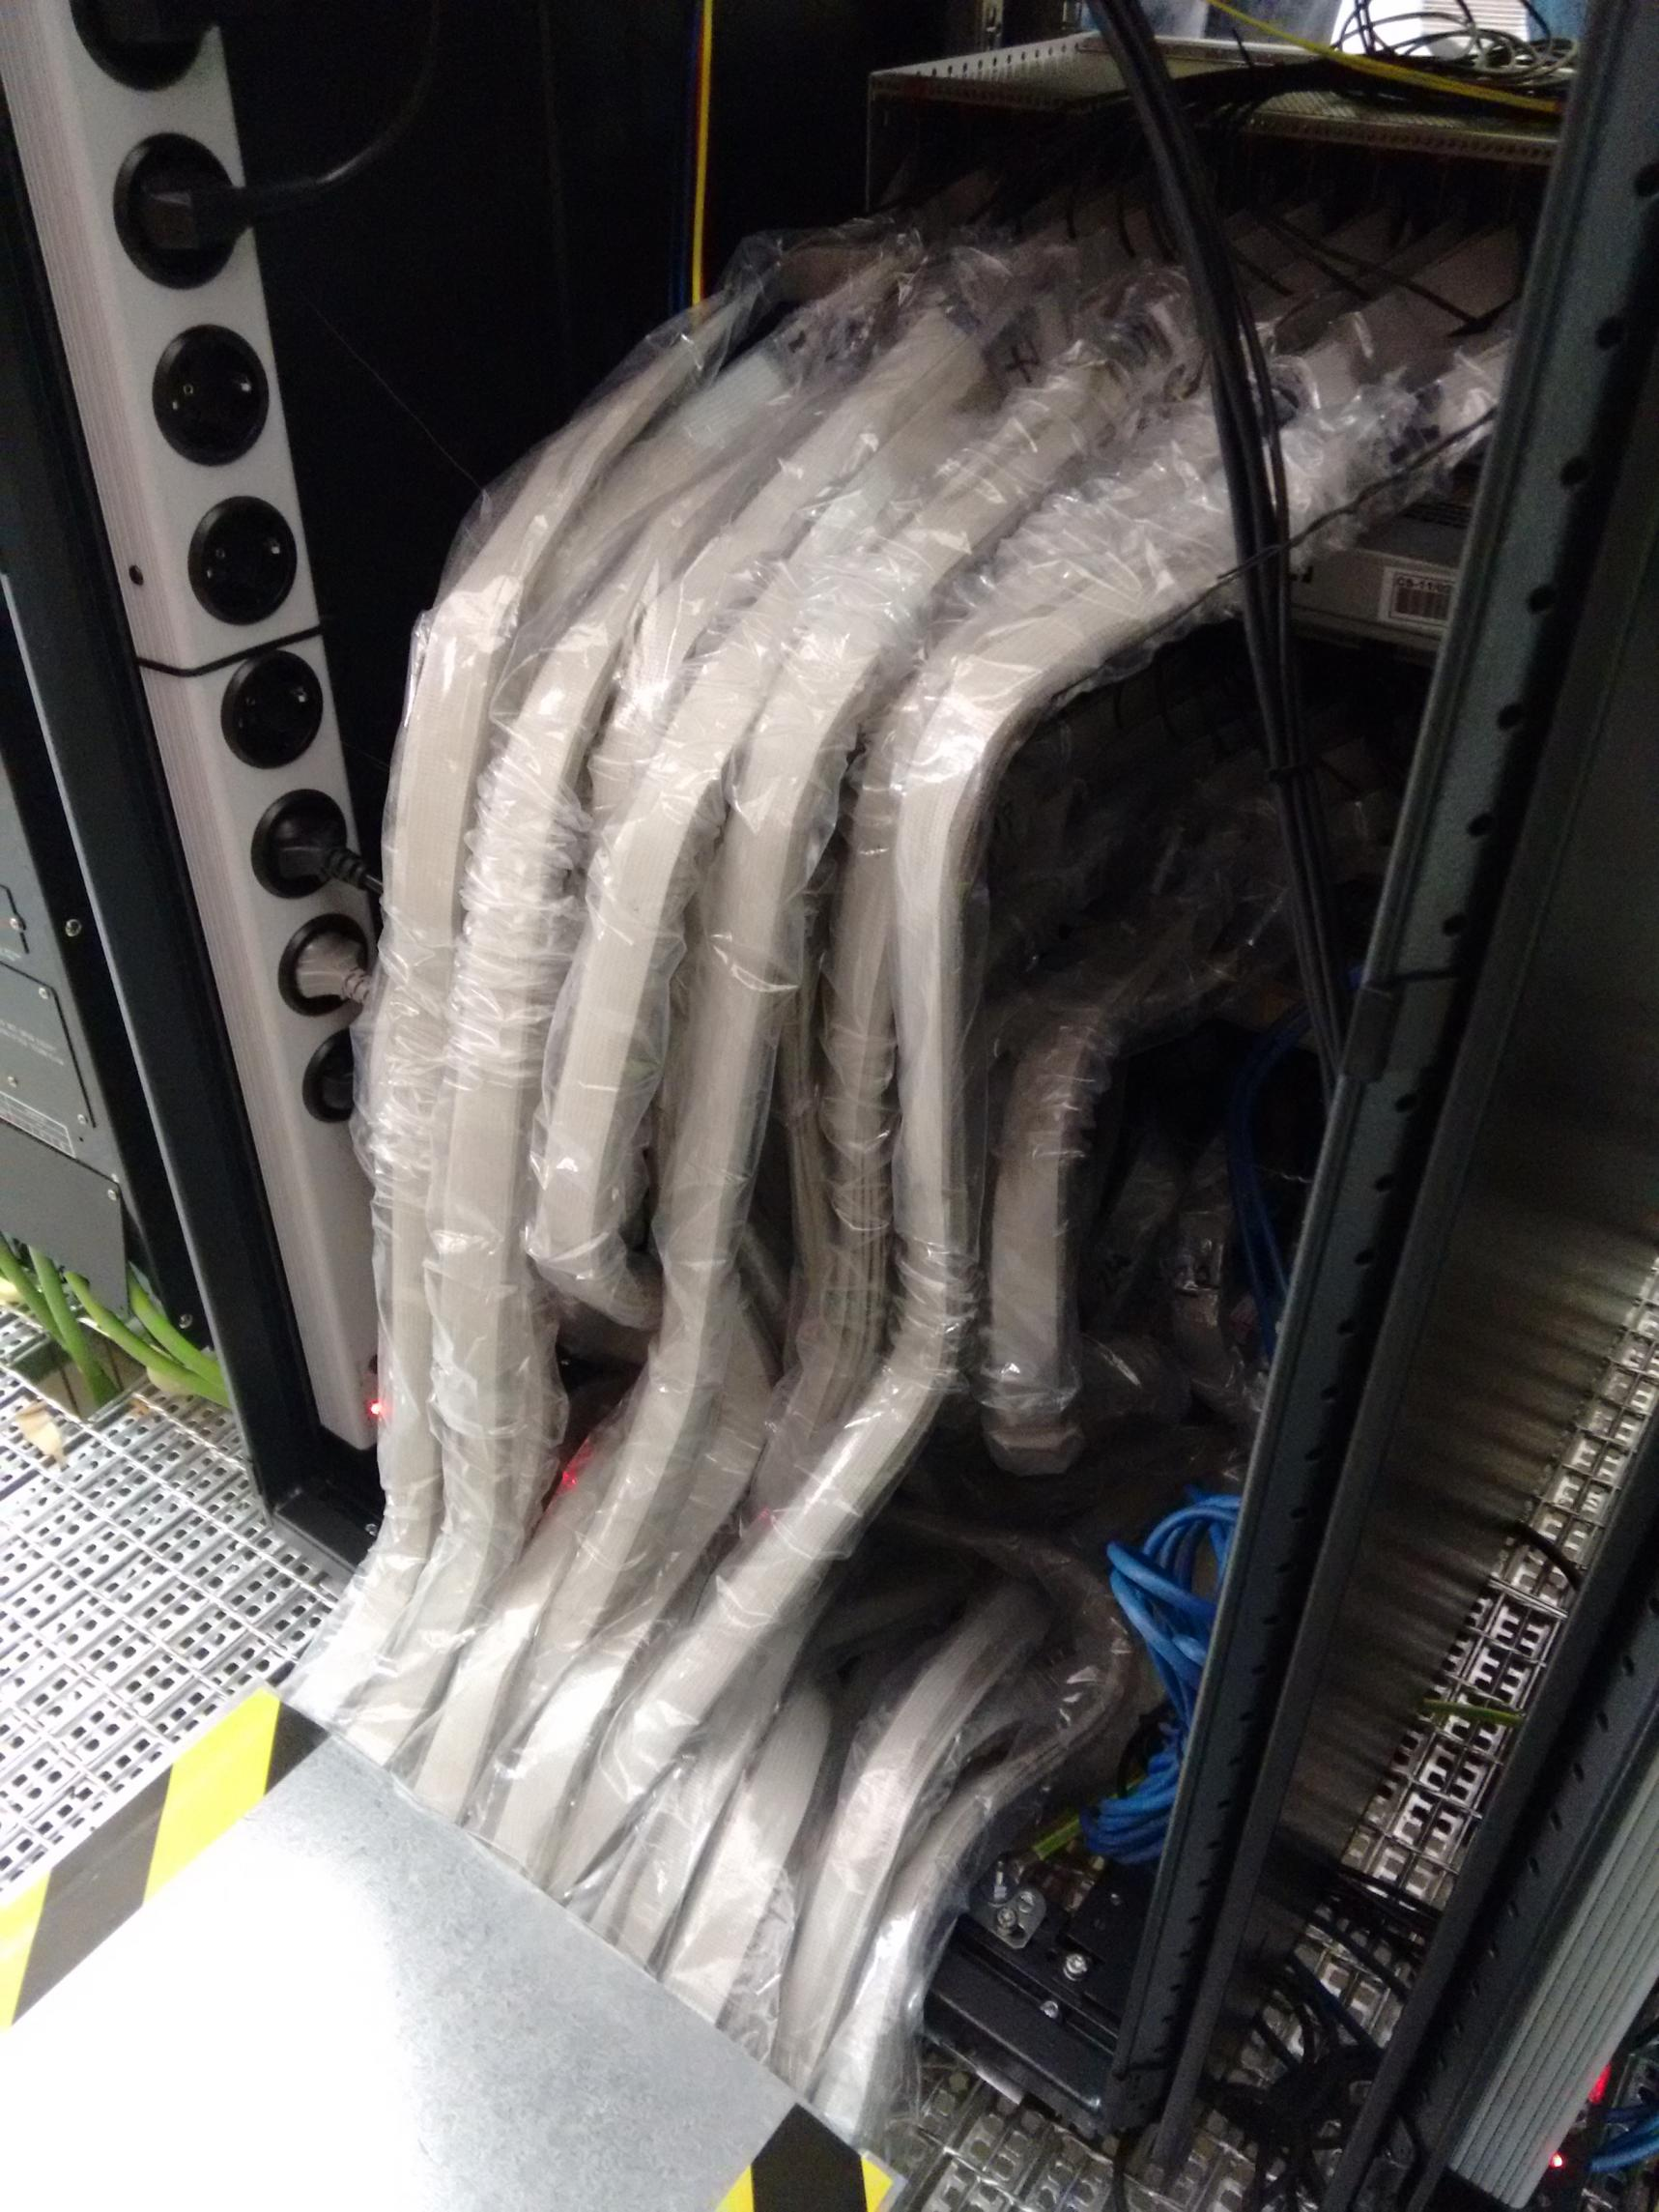
\includegraphics[width=.45\textwidth]{IMG/cabling2FEE}
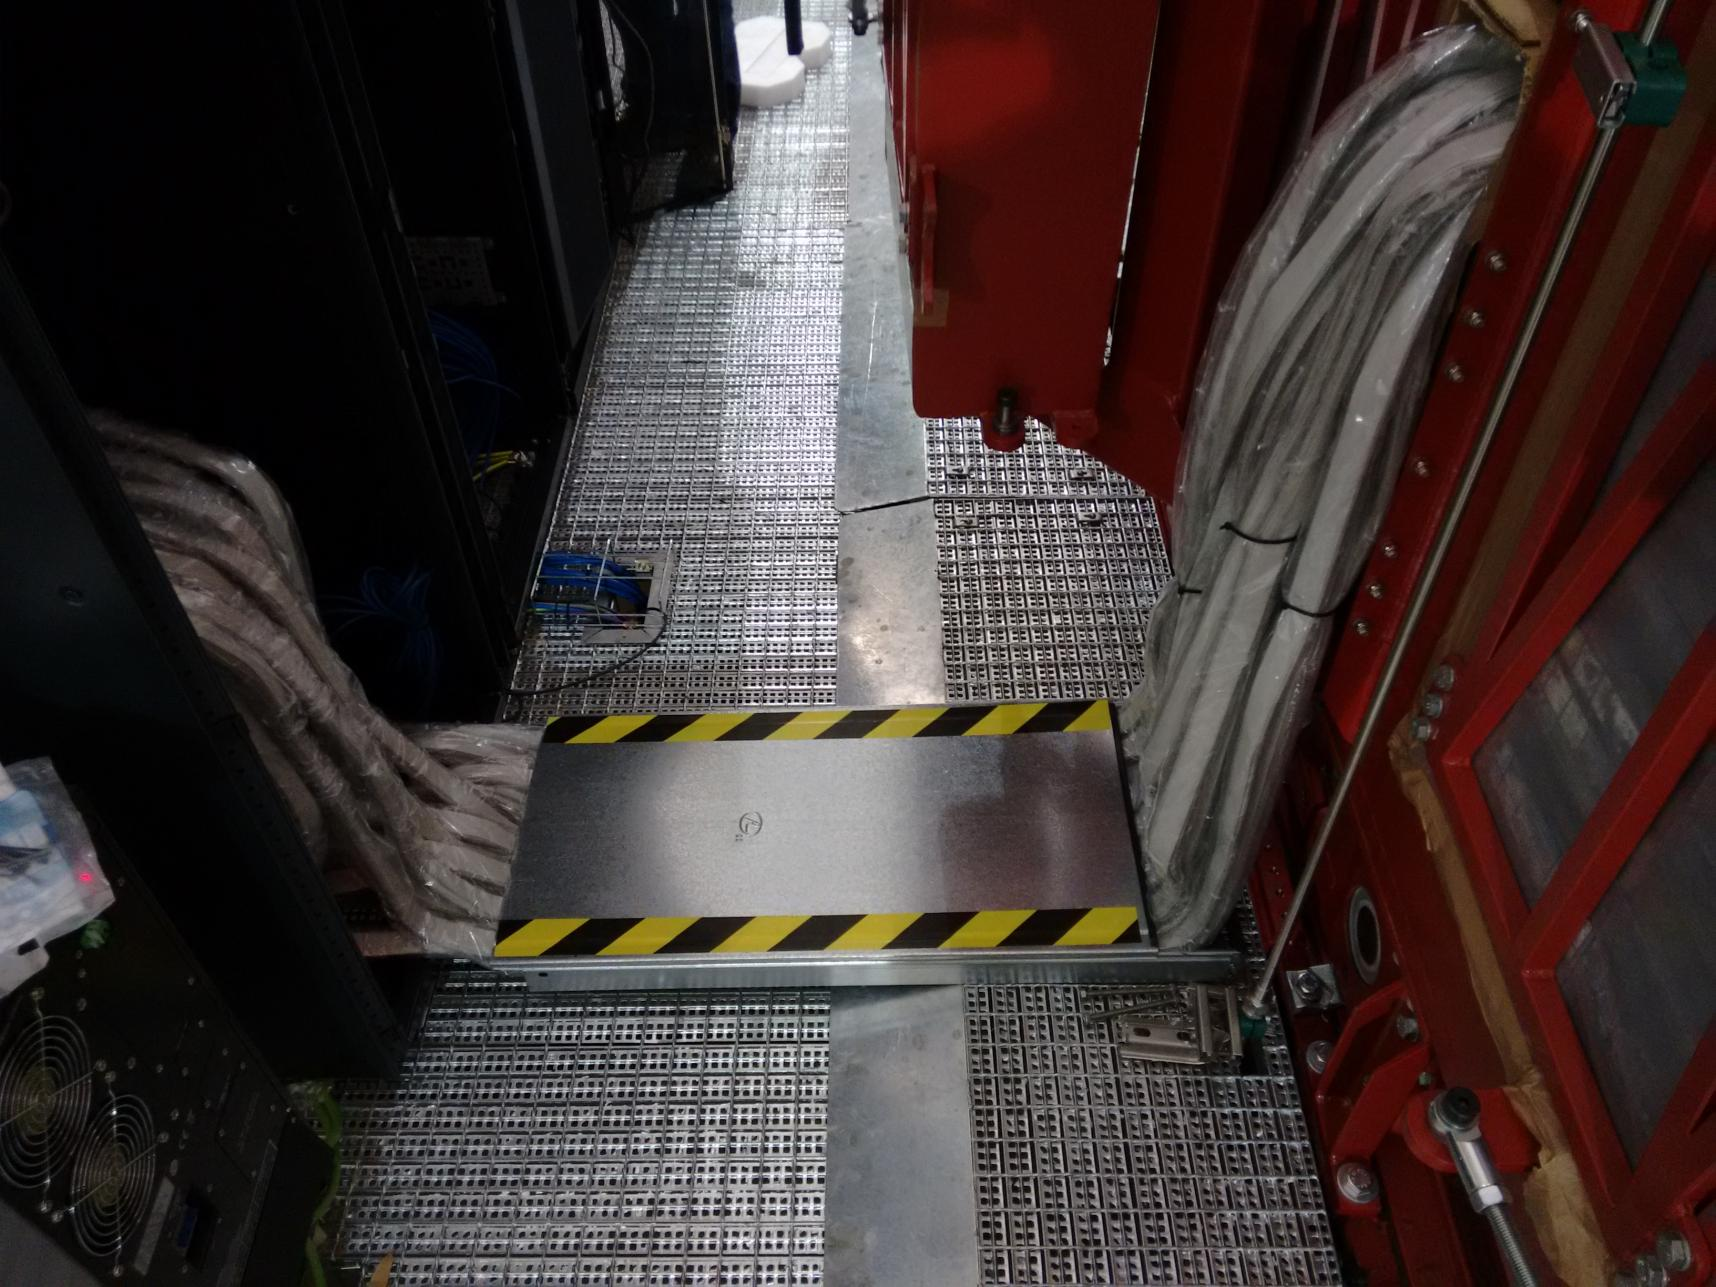
\includegraphics[width=.45\textwidth]{IMG/cabling_under_platform}
\caption{Different parts of the external cabling of the tracking plane. Up left shows a general view of the cabling. Up right picture is a detail of the connexion of the cables to the FEE boards. Bottom picture shows how the cables move under the platform.}
\label{fig:external_installation}
\end{figure}
